\documentclass[12pt]{article}

% Specify how big is going to be the paper margins.
\usepackage[a4paper, margin=1in]{geometry}

% amsmath: Add useful commans like aligh and gather.
% amsfonts: Add useful fonts like \mathbb{R}.
% amssymb: Add useful symbles like \therefore (needs amsfonts to work).
\usepackage{amsmath, amsfonts, amssymb}

% Makes the use of colors possible.
\usepackage{xcolor}

\definecolor{color1}{HTML}{0e4a7a}
\definecolor{color2}{HTML}{1282d6}
\definecolor{color3}{HTML}{7ac1ff}

% Add Latin Modern Fonts like Sans-serif and Roman.
\usepackage{lmodern}

% Makes header and footer configurable.
\usepackage{fancyhdr}

% Makes the use of colored and configured tables possible
\usepackage[most]{tcolorbox}

% Add commands to specify theorems like \newtheorem{x}{y}.
\usepackage{amsthm}

% Enables enumeration of items.
\usepackage{enumitem}

% Enables adding images.
\usepackage{graphicx}

% Enables cool hyper references.
\usepackage[colorlinks=true, linkcolor=color2, urlcolor=color2, citecolor=color2]{hyperref}

\title{\sffamily\bfseries{Soluções OMpD 2023 N2 Fase 1}}
\author{Samuel de Araújo Brandão}
\date{5 de Setembro de 2025}

\pagestyle{fancy}
\fancyhf{}

\fancyhead[L]{\sffamily\bfseries{Soluções OMpD 2023 N2 Fase 1}}
\fancyhead[R]{\textcolor{color2}{Samuel Brandão}, 5 de Setembro de 2025}
\fancyfoot[C]{\thepage}
\setlength{\headheight}{14.5pt}

\tcbset{
  statementbox/.style = {
    enhanced,
    width=\textwidth,
    title={Enunciado},
    title filled,
    fonttitle=\sffamily\bfseries,
    coltitle=white,
    colbacktitle=color1,
    colback=white,
    colframe=color1,
    boxrule=1pt,
    arc=2mm,
    boxsep=2pt,
  }
}

\tcbset{
  theorembox/.style = {
    enhanced,
    width=\textwidth,
    colback=white,
    colframe=color1,
    boxrule=1pt,
    arc=2mm,
    boxsep=2pt
  }
}

\tcbset{
  lemmabox/.style = {
    enhanced,
    width=\textwidth,
    colback=white,
    colframe=color2,
    boxrule=1pt,
    arc=2mm,
    boxsep=2pt
  }
}

\renewcommand*\contentsname{\textsf{Conteúdos}}
\newcommand{\kb}[1]{\left\lfloor #1 \right\rfloor}

\begin{document}
  \maketitle
  Uma coleção de soluções para a \textbf{OMpD 2023 Nível 2 Fase 1}, inspirada no estilo de Evan Chen.
  Pode-se encontrar todos os problemas \textbf{\href{https://drive.google.com/file/d/1OrSQW4Ykh-TRShUsfWR7WDy5UTMngq2x/view}
  {aqui}} e as respostas oficiais \textbf{\href{https://drive.google.com/file/d/1ShpN6c-oEayureeyQcHpztjcPC7zP8k_/view}{aqui}}.

  Todas as soluções foram inteiramente escritas por mim, enquanto me preparava para a
  International Mathematical Olympiad (IMO).

  Caso encontre algum erro ou tiver sugestões ou comentários, sinta-se a vontade 
  para entrar em contato!

  \tableofcontents

  \clearpage

  \section{\textsf{Problemas}}
    \begin{enumerate}[label=\textbf{{\arabic*.}}]
      \item Um vendedor comprou $1000$ bombons pelo preço de cinco por $2$ reais. Se ele vender todos esses bombons pelo preço de dois por $1$ real, qual será o lucro desse vendedor, em reais?

(A) 100 (B) 200 (C) 300 (D) 400 (E) 500

\item Seja $ABCDE$ um pentágono regular. Externamente a esse pentágono, construímos o triângulo equilátero $ABX$, e internamente a esse pentágono construímos o quadrado $EAYZ$, conforme a figura a seguir. Qual a medida do ângulo $\angle AXY$?

  \begin{center}
    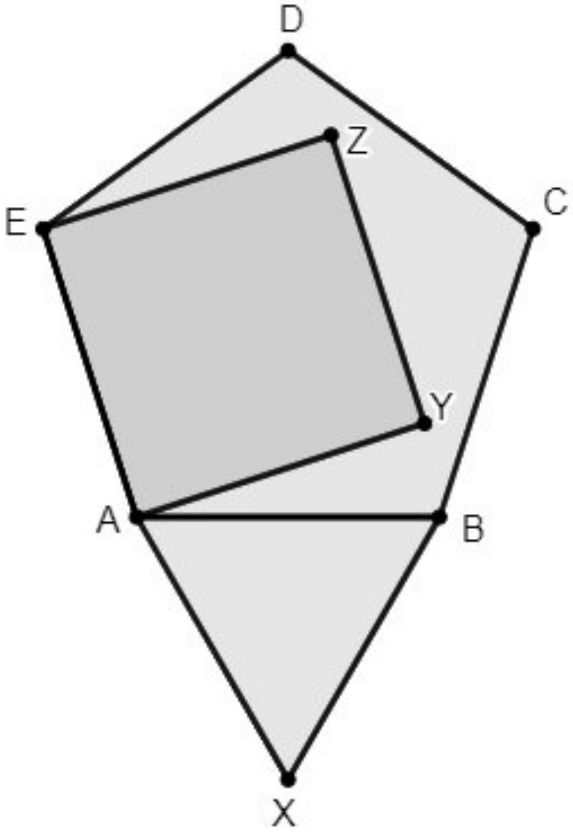
\includegraphics[width=0.2\textwidth]{first.png}
  \end{center}

(A) $9^\circ$ (B) $19^\circ$ (C) $21^\circ$ (D) $39^\circ$ (E) $51^\circ$

\item Dizemos que um inteiro positivo de $3$ algarismos é alternante se quaisquer dois algarismos consecutivos possuem paridades distintas. Por exemplo, $123$, $703$ e $494$ são alternantes, mas $231$, $772$ e $034$ não são alternantes. Quantos números alternantes existem?

(A) 200 (B) 225 (C) 250 (D) 275 (E) 300

\item Na multiplicação a seguir, cada quadradinho representa um algarismo não nulo.

    \begin{center}
    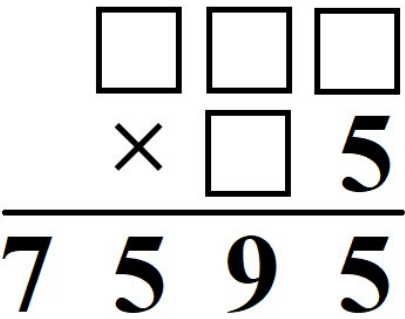
\includegraphics[width=0.1\textwidth]{second.png}
  \end{center}


Qual é a soma dos algarismos nos quadradinhos?
(A) 13 (B) 14 (C) 15 (D) 16 (E) 17

\item Na Escola Matemáticos por Diversão, há exatamente $500$ estudantes que estão ou no $8^\circ$ ano ou no $9^\circ$ ano. Sabemos que exatamente $40\%$ dos estudantes do $9^\circ$ ano gostam de álgebra, enquanto exatamente $30\%$ dos estudantes do $8^\circ$ ano não gostam de álgebra. Ao todo, exatamente $234$ de todos esses $500$ estudantes não gostam de álgebra. Quantos alunos do $8^\circ$ ano gostam de álgebra?

(A) 66 (B) 154 (C) 186 (D) 220 (E) 266

\item Entre os números naturais de $1$ até $n$, inclusive, pelo menos $13$ deles são divisíveis por $7$, e no máximo $11$ deles são divisíveis por $8$. Quantos desses números são divisíveis por $9$?

(A) 7 (B) 8 (C) 9 (D) 10 (E) 11

\item Lavi Dopes deseja caminhar sobre o plano. Partindo do ponto $A$, ele anda $5$ metros para o norte, depois $4$ metros para o leste, depois $3$ metros para o sul, depois $2$ metros para o oeste e, finalmente, $1$ metro para o norte, chegando assim no ponto $B$. Podemos afirmar que a distância entre os pontos $A$ e $B$ é:
(A) Maior que 2 metros e menor que 2,5 metros.
(B) Maior que 2,5 metros e menor que 3 metros.
(C) Maior que 3 metros e menor que 3,5 metros.
(D) Maior que 3,5 metros e menor que 4 metros.
(E) Maior que 4 metros.

\item De quantas maneiras podemos cobrir um tabuleiro $5\times 5$ com um quadrado de lado $3$, um quadrado de lado $2$ e três peças idênticas que fazem um L, cada uma ocupando quatro casinhas do tabuleiro? O tabuleiro não pode ser rotacionado, ou seja, as duas possibilidades a seguir devem ser consideradas distintas:

    \begin{center}
    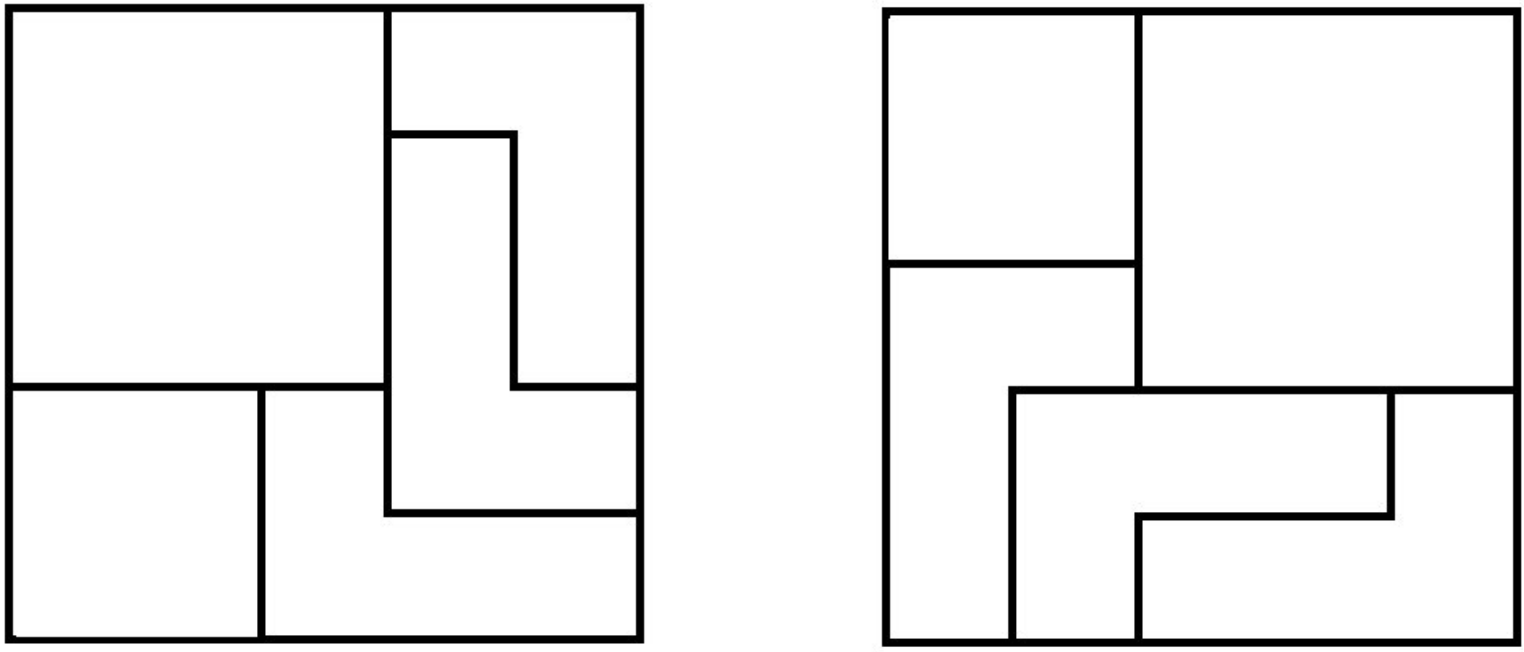
\includegraphics[width=0.3\textwidth]{third.png}
  \end{center}


(A) 4 (B) 8 (C) 12 (D) 16 (E) 24

\item Seja $ABCDEF$ um hexágono regular de área $24$ cm$^{2}$. Sejam $M$ e $P$ os pontos médios dos lados $\overline{AB}$ e $\overline{AF}$. Qual é a área do triângulo $MPD$?

(A) 9 cm$^{2}$ (B) 7 cm$^{2}$ (C) 6 cm$^{2}$ (D) 5 cm$^{2}$ (E) 3 cm$^{2}$

\item Link está brincando com seus superpoderes recém-adquiridos e decide usar a habilidade “Ascend” para alcançar o topo de um labirinto. Para isso, ele usa tal habilidade para sair do nível onde está e alcançar o chão de alguma sala no nível imediatamente superior, sem passar por paredes que separam salas num mesmo nível horizontal. As figuras 1 e 2 mostram duas maneiras distintas de Link alcançar o topo.

    \begin{center}
    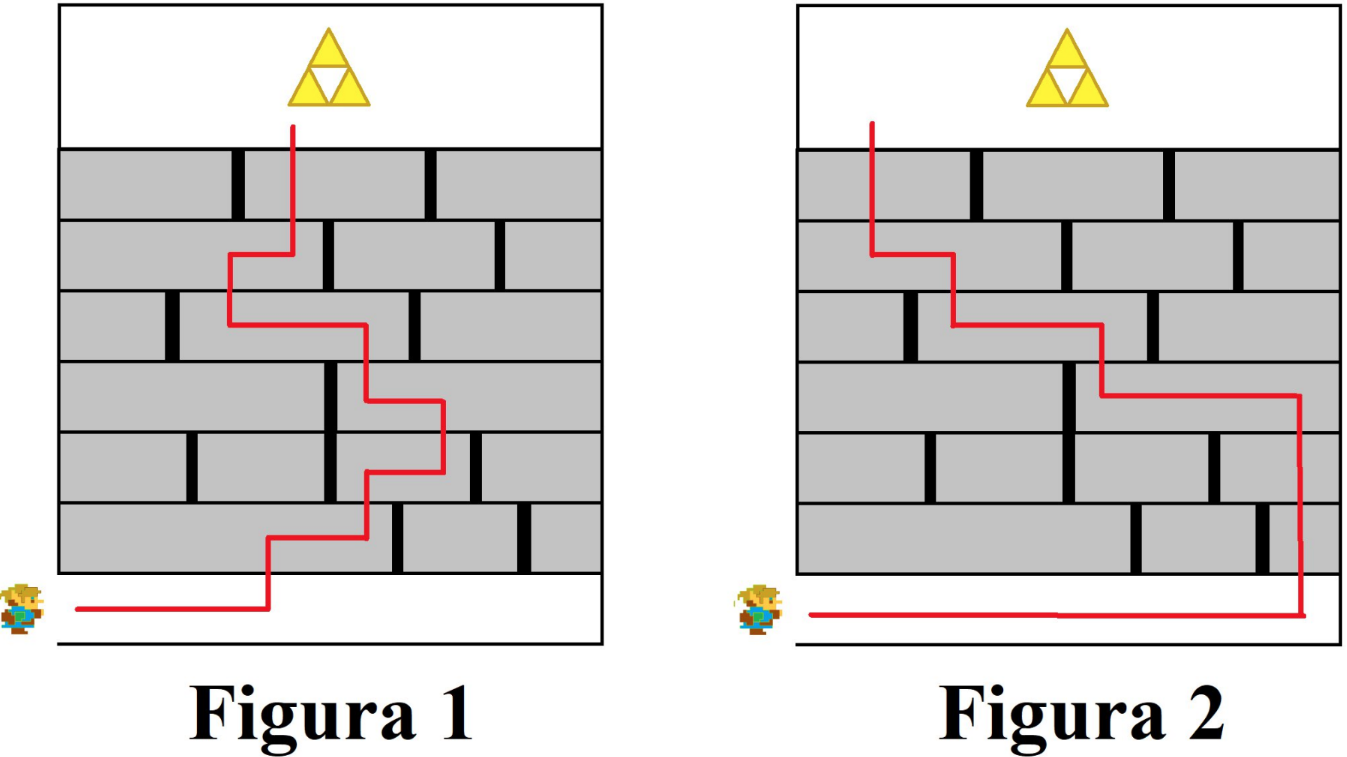
\includegraphics[width=0.4\textwidth]{fourth.png}
  \end{center}


Note que em cada maneira levamos em conta apenas quais das 18 salas Link visitou, de modo que duas maneiras são distintas se há ao menos uma sala visitada diferente em cada uma delas. De quantas maneiras Link pode alcançar o topo?
(A) 27 (B) 32 (C) 35 (D) 40 (E) 49

\item Luca dirige de sua casa até o aeroporto para ir à Semana Olímpica por meio de uma estrada em linha reta. Ele dirige 35 quilômetros em sua primeira hora, em velocidade constante, mas percebe que se continuar assim, chegará uma hora depois do planejado. Luca decide então pisar no acelerador, aumentando sua velocidade em 15 quilômetros por hora até o fim da viagem, e acaba chegando ao aeroporto meia hora antes do planejado. Qual a distância, em quilômetros, da casa de Luca até o aeroporto?

(A) 140 (B) 175 (C) 210 (D) 245 (E) 280

\item Dizemos que um inteiro positivo $n>1$ é intrigante se ele é igual a 119 vezes seu maior divisor primo. Por exemplo, 2023 é intrigante, pois $2023 = 119 \times 17$ e $17$ é seu maior divisor primo. Quantos inteiros positivos menores que 10000 são intrigantes?

(A) 1 (B) 5 (C) 9 (D) 13 (E) 17

\item Ana, Bernardo, Caíque, Davi e Enzo brincam de Werewolf. Dentre eles, há 3 aldeões, 1 lobo e 1 intruso. As afirmações de cada jogador foram as seguintes: \\
Ana: Caíque é aldeão. \\
Bernardo: Davi e Enzo não são ambos aldeões. \\
Caíque: Enzo é intruso. \\
Davi: Bernardo não é lobo. \\
Enzo: Ana e Bernardo não são ambos aldeões. \\
Sabendo que aldeões nunca mentem, e que o lobo e o intruso podem mentir, mas também podem falar a verdade, pode-se afirmar sempre que:
(A) Ana é lobo. (B) Bernardo é intruso. (C) Caíque é aldeão. (D) Davi é lobo. (E) Enzo não é intruso.

\item Inicialmente, temos um tabuleiro $3\times 3$, com um número $0$ escrito em cada um dos 9 quadradinhos. Uma operação consiste em escolher 4 quadradinhos que compartilham um mesmo vértice e somar 1 a cada um deles. Por exemplo, podemos realizar a sequência de operações a seguir:

      \begin{center}
    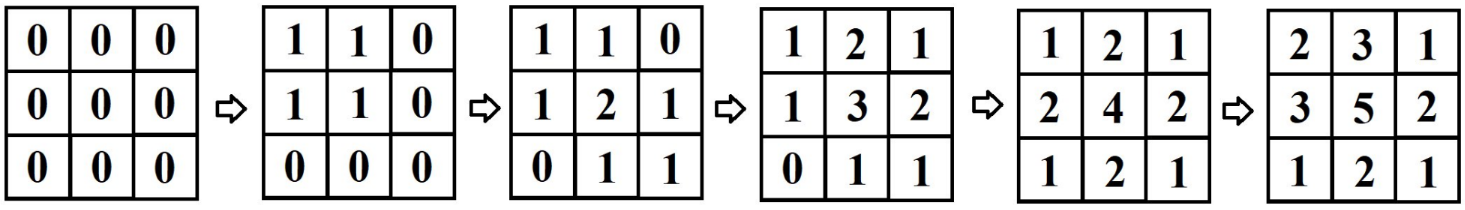
\includegraphics[width=0.8\textwidth]{fifth.png}
  \end{center}


Partindo do tabuleiro $3\times 3$ como 9 zeros, qual dos tabuleiros a seguir podemos obter após um número finito de operações?
    \begin{center}
    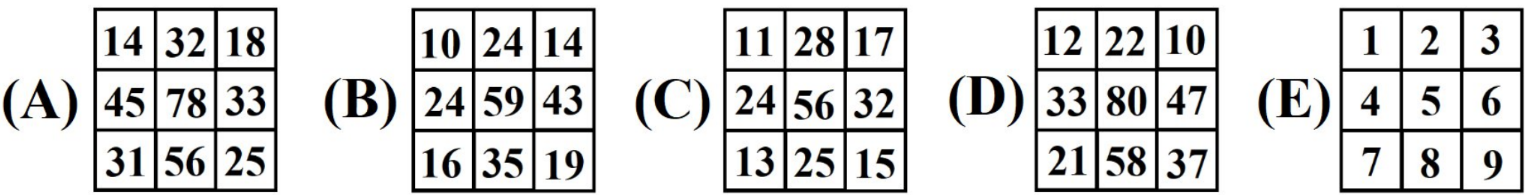
\includegraphics[width=0.8\textwidth]{sixth.png}
  \end{center}


\item Seja $ABCD$ um quadrilátero tal que $AD = BC$, $DB = DC$ e os lados $AB$ e $CD$ são paralelos. Se $AB = 16$ e $CD = 25$, qual é a medida de $AD$?

(A) 15 (B) 20 (C) 25 (D) 32 (E) 40

\item Certa vez, tartarugas e zumbis fizeram um rolezinho aleatório. Se cada tartaruga comprasse uma tortuguita e cada zumbi comprasse uma plutonita, eles gastariam ao todo 20 reais a mais do que se cada tartaruga comprasse uma plutonita e cada zumbi comprasse uma tortuguita. Sabendo que há mais tartarugas do que zumbis nesse rolezinho, e que o preço de cada comida é um número inteiro de reais, qual dos valores a seguir não pode ser um possível valor da quantidade de tartarugas a mais do que zumbis.

(A) 1 (B) 2 (C) 3 (D) 4 (E) 5

\item Sejam $a,b,c$ números reais tais que $a^{5}b^{8}c^{13} = 32$ e $a^{8}b^{13}c^{21} = 128$. Qual é o valor de $ab\,c^{2}$?

(A) 1 (B) 2 (C) 4 (D) 8 (E) 16

\item Dizemos que um conjunto de inteiros positivos é triangular se ele possui três elementos distintos que são os lados de um triângulo de área positiva. Por exemplo, $2,3,5,7$ é triangular, pois $3,5,7$ são lados de um triângulo de área positiva. Já $1,2,4,6$ não é triangular, pois não é possível escolher três elementos distintos que formem triângulo de área positiva. Seja $n$ um inteiro positivo tal que todo subconjunto de 12 elementos de $1,2,3,\ldots,n$ é triangular. Qual é o maior valor possível de $n$?

(A) 143 (B) 144 (C) 232 (D) 233 (E) 345

\item Quantos inteiros positivos de 10 algarismos, todos eles distintos, são múltiplos de 11111?

(A) 1264 (B) 2842 (C) 3456 (D) 3840 (E) 11111

\item Seja $AMD$ um triângulo acutângulo e escaleno, com $\angle MAD = 48^\circ$, e seja $\Omega$ sua circunferência inscrita, isto é, a circunferência tangente aos seus três lados. O ponto $B$ é definido como a interseção das bissetrizes externas de $\angle AMD$ e $\angle ADM$. Seja $P$ um ponto sobre $\Omega$ tal que a reta $BP$ é tangente a $\Omega$ em $P$. Qual é a medida do ângulo $\angle MPD$?

(A) $106^\circ$ (B) $114^\circ$ (C) $122^\circ$ (D) $130^\circ$ (E) $138^\circ$

    \end{enumerate}

  \clearpage

  \section{\textsf{Soluções}}
\subsection{Problema 1}
\begin{tcolorbox}[statementbox]
      Um vendedor comprou $1000$ bombons pelo preço de cinco por $2$ reais. Se ele vender todos esses bombons pelo preço de dois por $1$ real, qual será o lucro desse vendedor, em reais?

(A) 100 (B) 200 (C) 300 (D) 400 (E) 500
\end{tcolorbox}
\clearpage

\subsection{Problema 2}
\begin{tcolorbox}[statementbox]
Seja $ABCDE$ um pentágono regular. Externamente a esse pentágono, construímos o triângulo equilátero $ABX$, e internamente a esse pentágono construímos o quadrado $EAYZ$, conforme a figura a seguir. Qual a medida do ângulo $\angle AXY$?

  \begin{center}
    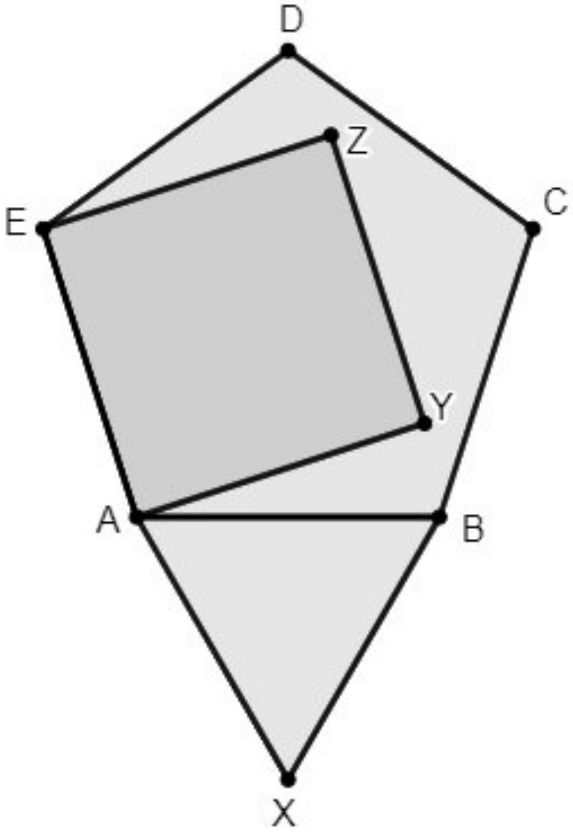
\includegraphics[width=0.2\textwidth]{first.png}
  \end{center}

(A) $9^\circ$ (B) $19^\circ$ (C) $21^\circ$ (D) $39^\circ$ (E) $51^\circ$
\end{tcolorbox}
\clearpage

\subsection{Problema 3}
\begin{tcolorbox}[statementbox]
Dizemos que um inteiro positivo de $3$ algarismos é alternante se quaisquer dois algarismos consecutivos possuem paridades distintas. Por exemplo, $123$, $703$ e $494$ são alternantes, mas $231$, $772$ e $034$ não são alternantes. Quantos números alternantes existem?

(A) 200 (B) 225 (C) 250 (D) 275 (E) 300
\end{tcolorbox}
\clearpage

\subsection{Problema 4}
\begin{tcolorbox}[statementbox]
Na multiplicação a seguir, cada quadradinho representa um algarismo não nulo.

    \begin{center}
    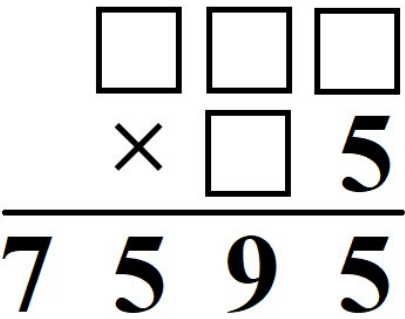
\includegraphics[width=0.1\textwidth]{second.png}
  \end{center}


Qual é a soma dos algarismos nos quadradinhos?
(A) 13 (B) 14 (C) 15 (D) 16 (E) 17
\end{tcolorbox}
\clearpage

\subsection{Problema 5}
\begin{tcolorbox}[statementbox]
Na Escola Matemáticos por Diversão, há exatamente $500$ estudantes que estão ou no $8^\circ$ ano ou no $9^\circ$ ano. Sabemos que exatamente $40\%$ dos estudantes do $9^\circ$ ano gostam de álgebra, enquanto exatamente $30\%$ dos estudantes do $8^\circ$ ano não gostam de álgebra. Ao todo, exatamente $234$ de todos esses $500$ estudantes não gostam de álgebra. Quantos alunos do $8^\circ$ ano gostam de álgebra?

(A) 66 (B) 154 (C) 186 (D) 220 (E) 266
\end{tcolorbox}
\clearpage

\subsection{Problema 6}
\begin{tcolorbox}[statementbox]
Entre os números naturais de $1$ até $n$, inclusive, pelo menos $13$ deles são divisíveis por $7$, e no máximo $11$ deles são divisíveis por $8$. Quantos desses números são divisíveis por $9$?

(A) 7 (B) 8 (C) 9 (D) 10 (E) 11
\end{tcolorbox}
\clearpage

\subsection{Problema 7}
\begin{tcolorbox}[statementbox]
Lavi Dopes deseja caminhar sobre o plano. Partindo do ponto $A$, ele anda $5$ metros para o norte, depois $4$ metros para o leste, depois $3$ metros para o sul, depois $2$ metros para o oeste e, finalmente, $1$ metro para o norte, chegando assim no ponto $B$. Podemos afirmar que a distância entre os pontos $A$ e $B$ é:
(A) Maior que 2 metros e menor que 2,5 metros.
(B) Maior que 2,5 metros e menor que 3 metros.
(C) Maior que 3 metros e menor que 3,5 metros.
(D) Maior que 3,5 metros e menor que 4 metros.
(E) Maior que 4 metros.
\end{tcolorbox}
\clearpage

\subsection{Problema 8}
\begin{tcolorbox}[statementbox]
De quantas maneiras podemos cobrir um tabuleiro $5\times 5$ com um quadrado de lado $3$, um quadrado de lado $2$ e três peças idênticas que fazem um L, cada uma ocupando quatro casinhas do tabuleiro? O tabuleiro não pode ser rotacionado, ou seja, as duas possibilidades a seguir devem ser consideradas distintas:

    \begin{center}
    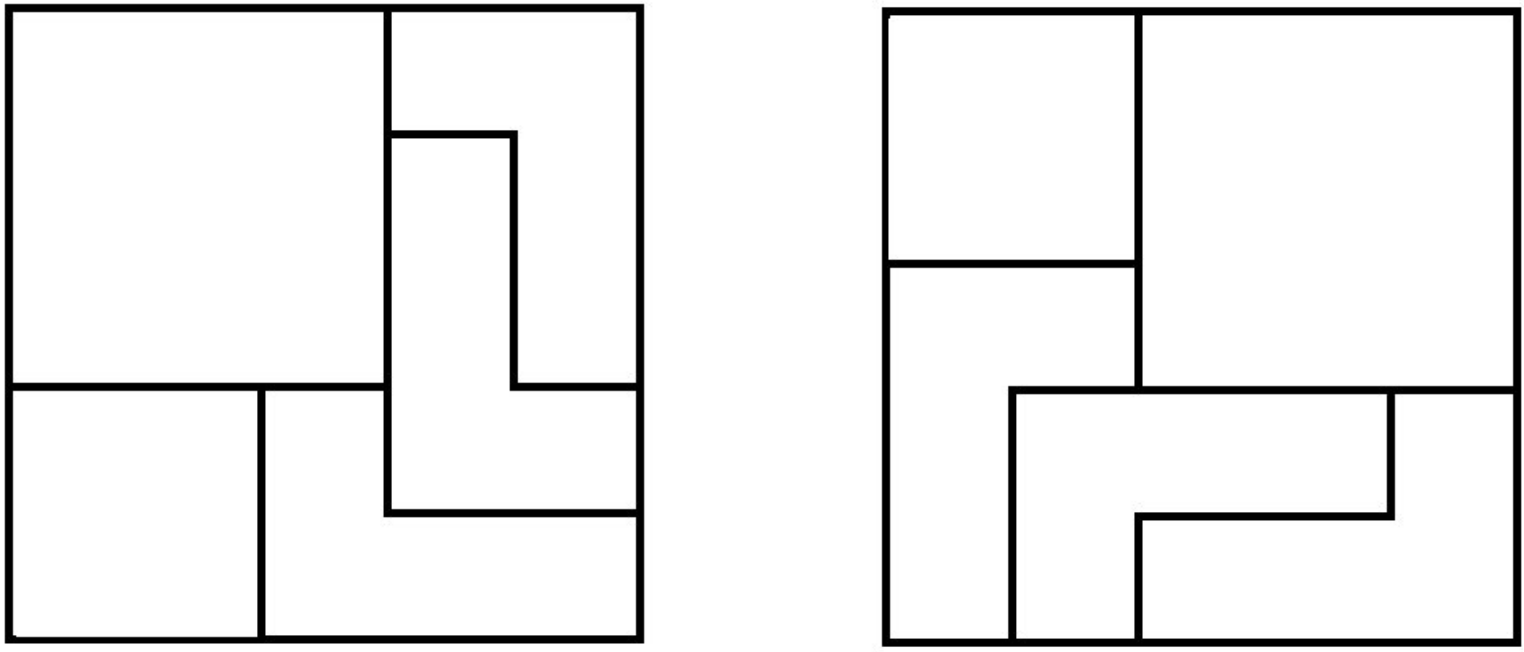
\includegraphics[width=0.3\textwidth]{third.png}
  \end{center}


(A) 4 (B) 8 (C) 12 (D) 16 (E) 24
\end{tcolorbox}
\clearpage

\subsection{Problema 9}
\begin{tcolorbox}[statementbox]
Seja $ABCDEF$ um hexágono regular de área $24$ cm$^{2}$. Sejam $M$ e $P$ os pontos médios dos lados $\overline{AB}$ e $\overline{AF}$. Qual é a área do triângulo $MPD$?

(A) 9 cm$^{2}$ (B) 7 cm$^{2}$ (C) 6 cm$^{2}$ (D) 5 cm$^{2}$ (E) 3 cm$^{2}$
\end{tcolorbox}
\clearpage

\subsection{Problema 10}
\begin{tcolorbox}[statementbox]
Link está brincando com seus superpoderes recém-adquiridos e decide usar a habilidade “Ascend” para alcançar o topo de um labirinto. Para isso, ele usa tal habilidade para sair do nível onde está e alcançar o chão de alguma sala no nível imediatamente superior, sem passar por paredes que separam salas num mesmo nível horizontal. As figuras 1 e 2 mostram duas maneiras distintas de Link alcançar o topo.

    \begin{center}
    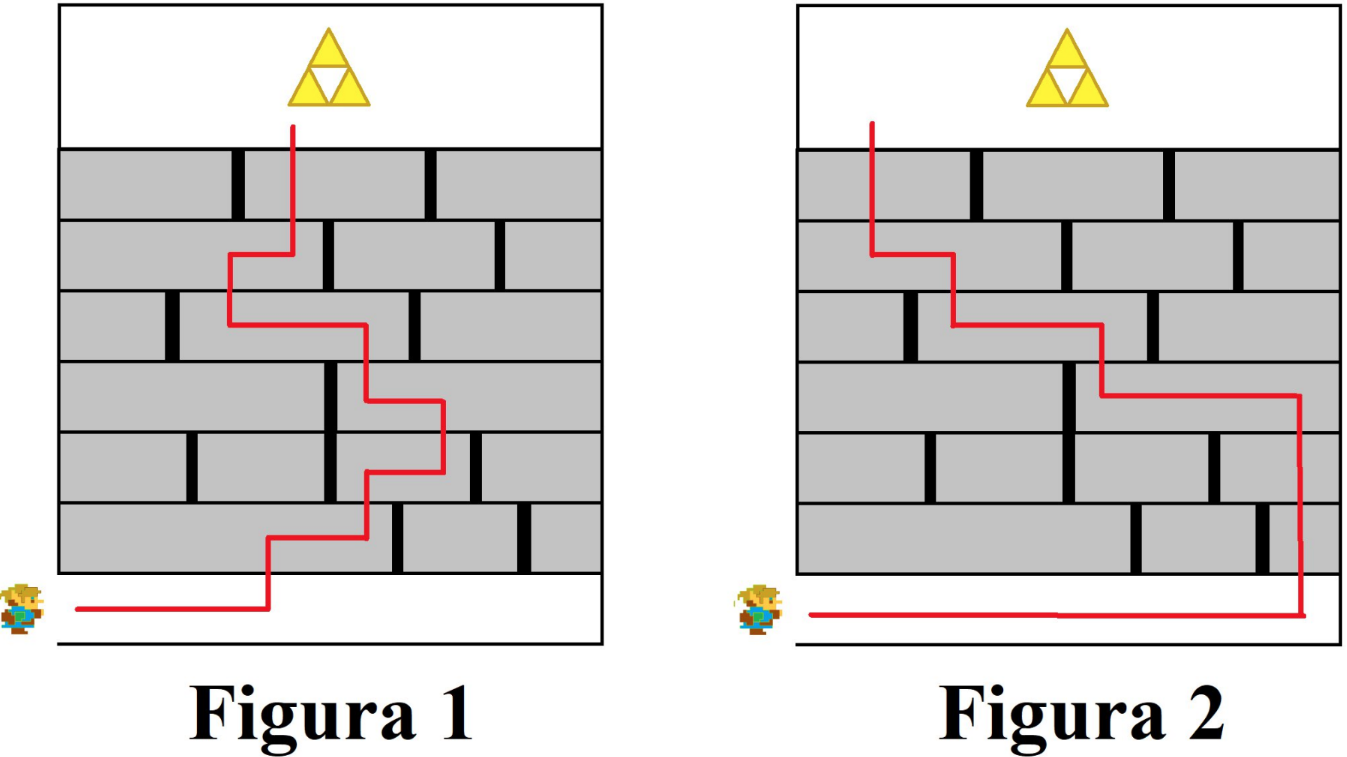
\includegraphics[width=0.4\textwidth]{fourth.png}
  \end{center}


Note que em cada maneira levamos em conta apenas quais das 18 salas Link visitou, de modo que duas maneiras são distintas se há ao menos uma sala visitada diferente em cada uma delas. De quantas maneiras Link pode alcançar o topo?
(A) 27 (B) 32 (C) 35 (D) 40 (E) 49
\end{tcolorbox}
\clearpage

\subsection{Problema 11}
\begin{tcolorbox}[statementbox]
Luca dirige de sua casa até o aeroporto para ir à Semana Olímpica por meio de uma estrada em linha reta. Ele dirige 35 quilômetros em sua primeira hora, em velocidade constante, mas percebe que se continuar assim, chegará uma hora depois do planejado. Luca decide então pisar no acelerador, aumentando sua velocidade em 15 quilômetros por hora até o fim da viagem, e acaba chegando ao aeroporto meia hora antes do planejado. Qual a distância, em quilômetros, da casa de Luca até o aeroporto?

(A) 140 (B) 175 (C) 210 (D) 245 (E) 280
\end{tcolorbox}
\clearpage

\subsection{Problema 12}
\begin{tcolorbox}[statementbox]
Dizemos que um inteiro positivo $n>1$ é intrigante se ele é igual a 119 vezes seu maior divisor primo. Por exemplo, 2023 é intrigante, pois $2023 = 119 \times 17$ e $17$ é seu maior divisor primo. Quantos inteiros positivos menores que 10000 são intrigantes?

(A) 1 (B) 5 (C) 9 (D) 13 (E) 17
\end{tcolorbox}
\clearpage

\subsection{Problema 13}
\begin{tcolorbox}[statementbox]
Ana, Bernardo, Caíque, Davi e Enzo brincam de Werewolf. Dentre eles, há 3 aldeões, 1 lobo e 1 intruso. As afirmações de cada jogador foram as seguintes: \\
Ana: Caíque é aldeão. \\
Bernardo: Davi e Enzo não são ambos aldeões. \\
Caíque: Enzo é intruso. \\
Davi: Bernardo não é lobo. \\
Enzo: Ana e Bernardo não são ambos aldeões. \\
Sabendo que aldeões nunca mentem, e que o lobo e o intruso podem mentir, mas também podem falar a verdade, pode-se afirmar sempre que:
(A) Ana é lobo. (B) Bernardo é intruso. (C) Caíque é aldeão. (D) Davi é lobo. (E) Enzo não é intruso.
\end{tcolorbox}
\clearpage

\subsection{Problema 14}
\begin{tcolorbox}[statementbox]
Inicialmente, temos um tabuleiro $3\times 3$, com um número $0$ escrito em cada um dos 9 quadradinhos. Uma operação consiste em escolher 4 quadradinhos que compartilham um mesmo vértice e somar 1 a cada um deles. Por exemplo, podemos realizar a sequência de operações a seguir:

      \begin{center}
    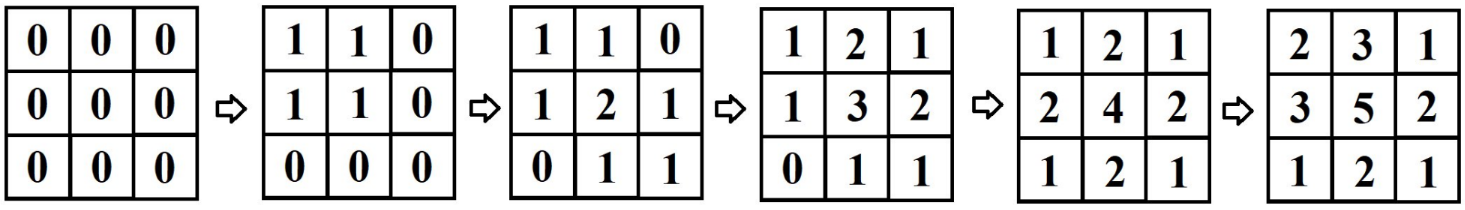
\includegraphics[width=0.8\textwidth]{fifth.png}
  \end{center}


Partindo do tabuleiro $3\times 3$ como 9 zeros, qual dos tabuleiros a seguir podemos obter após um número finito de operações?
    \begin{center}
    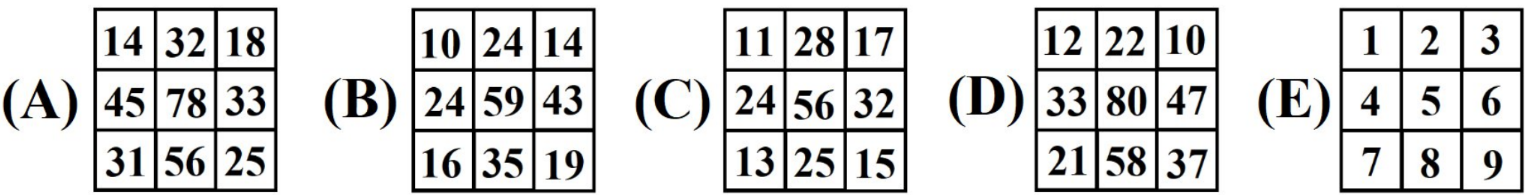
\includegraphics[width=0.8\textwidth]{sixth.png}
  \end{center}
\end{tcolorbox}
\clearpage

\subsection{Problema 15}
\begin{tcolorbox}[statementbox]
Seja $ABCD$ um quadrilátero tal que $AD = BC$, $DB = DC$ e os lados $AB$ e $CD$ são paralelos. Se $AB = 16$ e $CD = 25$, qual é a medida de $AD$?

(A) 15 (B) 20 (C) 25 (D) 32 (E) 40
\end{tcolorbox}
\clearpage

\subsection{Problema 16}
\begin{tcolorbox}[statementbox]
Certa vez, tartarugas e zumbis fizeram um rolezinho aleatório. Se cada tartaruga comprasse uma tortuguita e cada zumbi comprasse uma plutonita, eles gastariam ao todo 20 reais a mais do que se cada tartaruga comprasse uma plutonita e cada zumbi comprasse uma tortuguita. Sabendo que há mais tartarugas do que zumbis nesse rolezinho, e que o preço de cada comida é um número inteiro de reais, qual dos valores a seguir não pode ser um possível valor da quantidade de tartarugas a mais do que zumbis.

(A) 1 (B) 2 (C) 3 (D) 4 (E) 5
\end{tcolorbox}
\clearpage

\subsection{Problema 17}
\begin{tcolorbox}[statementbox]
Sejam $a,b,c$ números reais tais que $a^{5}b^{8}c^{13} = 32$ e $a^{8}b^{13}c^{21} = 128$. Qual é o valor de $ab\,c^{2}$?

(A) 1 (B) 2 (C) 4 (D) 8 (E) 16
\end{tcolorbox}
\clearpage

\subsection{Problema 18}
\begin{tcolorbox}[statementbox]
Dizemos que um conjunto de inteiros positivos é triangular se ele possui três elementos distintos que são os lados de um triângulo de área positiva. Por exemplo, $2,3,5,7$ é triangular, pois $3,5,7$ são lados de um triângulo de área positiva. Já $1,2,4,6$ não é triangular, pois não é possível escolher três elementos distintos que formem triângulo de área positiva. Seja $n$ um inteiro positivo tal que todo subconjunto de 12 elementos de $1,2,3,\ldots,n$ é triangular. Qual é o maior valor possível de $n$?

(A) 143 (B) 144 (C) 232 (D) 233 (E) 345
\end{tcolorbox}
\clearpage

\subsection{Problema 19}
\begin{tcolorbox}[statementbox]
Quantos inteiros positivos de 10 algarismos, todos eles distintos, são múltiplos de 11111?

(A) 1264 (B) 2842 (C) 3456 (D) 3840 (E) 11111
\end{tcolorbox}
\clearpage

\subsection{Problema 20}
\begin{tcolorbox}[statementbox]
Seja $AMD$ um triângulo acutângulo e escaleno, com $\angle MAD = 48^\circ$, e seja $\Omega$ sua circunferência inscrita, isto é, a circunferência tangente aos seus três lados. O ponto $B$ é definido como a interseção das bissetrizes externas de $\angle AMD$ e $\angle ADM$. Seja $P$ um ponto sobre $\Omega$ tal que a reta $BP$ é tangente a $\Omega$ em $P$. Qual é a medida do ângulo $\angle MPD$?

(A) $106^\circ$ (B) $114^\circ$ (C) $122^\circ$ (D) $130^\circ$ (E) $138^\circ$
\end{tcolorbox}
\clearpage

\clearpage


  \section{\textsf{Referências}}
\end{document}
